\begin{corr}{Magnétostatique}
\correction{Orage et boussole}
\begin{corrlist}
\item Voir figure~\ref{fig:magneto_spire}. On se place donc dans un repère cylindrique
      $(O, \er, \etheta, \ez)$. Un point $M$ est repéré par ses coordonnées 
      $(r, \theta, \phi)$.

\item  L'étude
      des invariances de la distribution de courant montre que la norme du 
      champ magnétique \fbox{ne dépend que de la distance au fil $r$}. L'étude des
      symétries montre que le champ magnétique est \fbox{orthoradial}.
      Les lignes de champ sont des \fbox{cercles concentriques} centrés le fil.

\item Voir cours. L'expression du champ magnétique en un point $M$ situé 
  à une distance $r$ du fil est donnée par
  \begin{equation*}
	  \vecb(M) = \dfrac{\mu_0 I}{2 \pi R} \etheta.
   \end{equation*}
   On vérifie la dimension de cette expression. D'après le théorème d'Ampère
   on sait que la circulation de $\vecb$ sur un contour fermé est égale à 
   $\mu_0 I$. Or la circulation de $\vecb$ est homogène à champ magnétique 
   multiplié par une longueur ($\vecb \cdot \dl$). L'expression est donc bien homogène.

   \item 
	   \begin{equation*}
		B(M) < B_L \iff \dfrac{\mu_0 I}{2 \pi r} < B_L \iff 
		r > \dfrac{\mu_0 I}{2 \pi B_L} \iff \boxed{r > \unit{10}{\meter}} 
	   \end{equation*}
	Si la boussole se trouve à moins de $\unit{10}{\meter}$ de l'éclair, 
	elle sera désaimantée.
\end{corrlist}


\correction{Bobines de Helmholtz}
	\begin{corrlist}
		\item On commence bien sûr par réaliser un schéma du système
			(voir Fig.~\ref{fig:spire_ex}).
		      On choisit d'utiliser dans cet exercice un repère cylindrique
		      $(O, \er, \etheta, \ez)$. Un point $M$ de l'axe $(Oz)$
		      est donc repéré par ses coordonnées $(0, 0, z)$. Sous
		      sa forme la plus générale, le champ magnétique en $M$ 
		      s'écrit 
		      \begin{equation*}
			      \vecb_1(M) = B_r(M) \er + B_\theta(M) \etheta +
			      B_z(M) \ez.
		      \end{equation*}

		      \begin{description}
			     \item[Invariance:] La distribution de courant est 
			     invariante par rotation autour de l'axe $(Oz)$, 
			     $B_1$ ne dépend donc pas de $\theta$. De plus, on 
			     s'intéresse à un point $M$ situé sur l'axe, la
			     distance $r$ à l'axe de la spire n'entre donc pas
			     en compte dans le problème.
		     \item[Symétrie: ] Tout plan contenant l'axe $(Oz)$ est 
			               plan d'antisymétrie de la distribution de courant,
				       $\vecb_1(M)$ doit donc appartenir à l'intersection
				       de tous ces plans. $\vecb_1(M)$ est donc colinéaire
				       à $\ez$.
		     \end{description}
		     Finalement,
		     \begin{equation*}
			     \boxed{\vecb_1(M) = B_z(z) \ez.}
		     \end{equation*}
		
		\item La première étape est de déterminer le champ magnétique généré
		  par une portion $\dl_P$ de la spire centrée au point $P$
		  de coordonnées $(R, \theta, 0)$.On commence donc par exprimer $\dl_P$ 
		  dans le système de coordonnées choisi
		  \begin{equation*}
			  \dl_P = R \dtheta \etheta.
		  \end{equation*}
		  Vient ensuite l'expression de $\mitbf{PM}$ 
		  dans ce même référentiel
		  \begin{equation*}
			  \mitbf{PM} = \mitbf{PO} + \mitbf{OM} = -R \er + z\ez.
		  \end{equation*}
		  On aboutit ainsi à l'expression du champ magnétique $
		  \mathrm{\textbf{d}}\vecb_P(M)$
		  généré par cette portion de spire en $M$
		  \begin{equation*}
			  \mathrm{\textbf{d}}\vecb_P(M) = \dfrac{\mu_0 I}{4 \pi} \times 
			  \dfrac{\dl_P \wedge \mitbf{PM}}{PM^3}
			  = \dfrac{\mu_0 I}{4 \pi} \times \dfrac{R^2\ez + Rz\er}
			  {\left(R^2 + z^2\right)^{3/2}} \dtheta.
		  \end{equation*}
		  Il ne reste finalement plus qu'à sommer les contributions 
		  de toutes les portions de la spire pour aboutir au champ total
		  $\vecb_1(M)$
		  \begin{equation*}
			  \vecb_1(M) = \int_0^{2\pi} \dfrac{\mu_0 I}{4 \pi} \times 
			  \dfrac{R^2\ez + Rz\er}
			  {\left(R^2 + z^2\right)^{3/2}} \dtheta
			  = \dfrac{\mu_0 I}{4 \pi\left(R^2 + z^2\right)^{3/2}} 
			  \left(
		            R^2\ez  
		    \int_0^{2\pi}\dtheta + Rz \int_0^{2\pi} \er \dtheta
		     \right)
		     = \dfrac{\mu_0 I R^2}{2 \left(R^2 + z^2\right)^{3/2}}\ez.
		  \end{equation*}
		  $B_0$ est le champ obtenu en $z = 0$, il vaut donc
		  \begin{equation*}
			  B_0 = \dfrac{\mu_0 I}{2 R}.
		  \end{equation*}
		  On obtient finalement
		  \begin{equation*}
			  \boxed{\vecb_1(M) = B_0 \times 
			  \left[1 + \left(\dfrac{z}{R}\right)^2\right]^{-3/2}\ez.}
		  \end{equation*}
		  La figure~\ref{fig:helmholtz} représente l'évolution de 
		  $B(M)/B_0$ avec $z/R$.
		  \begin{figure}[htpb]
		  	\centering
			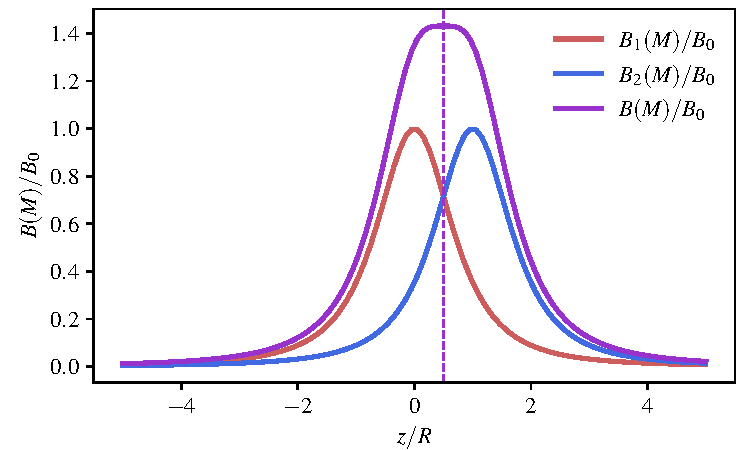
\includegraphics[scale=0.8]{helmholtz}
			\caption{$B_1(M)/B_0$, $B_2(M)/B_0$ et $B(M)/B_0$ 
			         en fonction de $z/R$. La ligne en pointillé correspond
			 à l'abscisse $z/R = 1/2$.}%
			\label{fig:helmholtz}
		  \end{figure}

	  \item On ajoute ensuite une seconde spire qui génère en $M$ un champ magnétique
		$\vecb_2(M)$. La spire $2$ étant identique à la première, on écrit
		directement que
		\begin{equation*}
			\vecb_2(M) = B_0 \times \left[1 + \left(\dfrac{z - R}{R}\right)^2
			\right]^{-3/2}\ez.
		\end{equation*}
		En utilisant le principe de superposition, on en déduit le champ
		magnétique total $\vecb$ généré en $M$
		\begin{equation*}
			\boxed{\vecb(M) = \vecb_1(M) + \vecb_2(M) 
			         = B_0 \left\{\left[1 + \left(\dfrac{z}{R}\right)^2
				 \right]^{-3/2} + \left[1 + \left(\dfrac{z-R}{R}\right)^2
	 \right]^{-3/2}\right\} \ez.}
		\end{equation*} 
		La figure~\ref{fig:helmholtz} trace l'évolution de $B(M)/B_0$ 
		en fonction de $z/R$. On remarque sur cette figure que la fonction est
		constante autour de $R/2$. Les lignes de champ seront donc \fbox{parallèles}
		autour de ce point.

	\end{corrlist}


\begin{figure}[htpb]
	\centering
	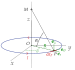
\includegraphics[scale=0.75]{spire}
	\caption{Schéma de la spire.}%
	\label{fig:spire_ex}
\end{figure}
\correction{Effet Meissner}
\begin{corrlist}
	\item On sait d'après l'équation de Maxwell-Ampère que 
	\begin{equation*}
		\rot \vecb = \mu_0 \vecj.
	\end{equation*}
	$\mu_0 \rot \vecj$ est donc homogène à un champ magnétique divisé par le carré
	d'une longueur. \fbox{$\lambda$ est donc homogène à une longueur.}

	\item D'après l'équation de Maxwell-Ampère, on a
	\begin{equation*}
		\rot \vecb = \mu_0 \vecj \Rightarrow \rot(\rot \vecb) = \mu_0 \rot \vecj.
	\end{equation*}
	En utilisant l'équation de London et l'égalité vectoriel fournie cela donne
	\begin{equation*}
		\rot(\rot \vecb) = -\dfrac{\vecb}{\lambda^2} \iff
		\gradient(\div \vecb) - \laplacien(\vecb) = -\dfrac{\vecb}{\lambda^2}.
	\end{equation*}
	En utilisant l'équation de Maxwell-Thomson, $\div \vecb = 0$, on aboutit ainsi à
	\begin{equation*}
		\boxed{\dd{^2B}{x^2} - \dfrac{B}{\lambda^2} = 0.}
	\end{equation*}

	\item $C$ doit obligatoirement être nul. Dans le cas contraire l'amplitude du
	      champ magnétique divergerait lorsque $x$ tend vers $\infty$. Pour déterminer $D$,
	      on utilise la continuité du champ en $x = 0$. On a donc directement
	      \begin{equation*}
		      \boxed{\vecb(x) = B_0 \exp\left(\dfrac{-x}{\lambda}\right)\ez.}
	      \end{equation*}
	
	\item
	\begin{equation*}
	     \begin{array}{c|lll}
			x	& \lambda & 10\lambda & 100\lambda \\[0.3em] \hline \\[0.2em]
			B(x)/B_0 & 0.37    & 4.5 \times 10^{-5} & 3.7 \times 10^{-44} \\[1em]
	      \end{array}
	\end{equation*}

	     $\lambda$ correspond donc à la profondeur de pénétration de $\vecb$
	     dans le supraconducteur.
\end{corrlist}


\correction{Champ créé par un câble coaxial}
\begin{corrlist}
	\item Le système est représenté sur la figure~\ref{fig:magneto_coaxial}.
		\begin{figure}[h]
		\centering
		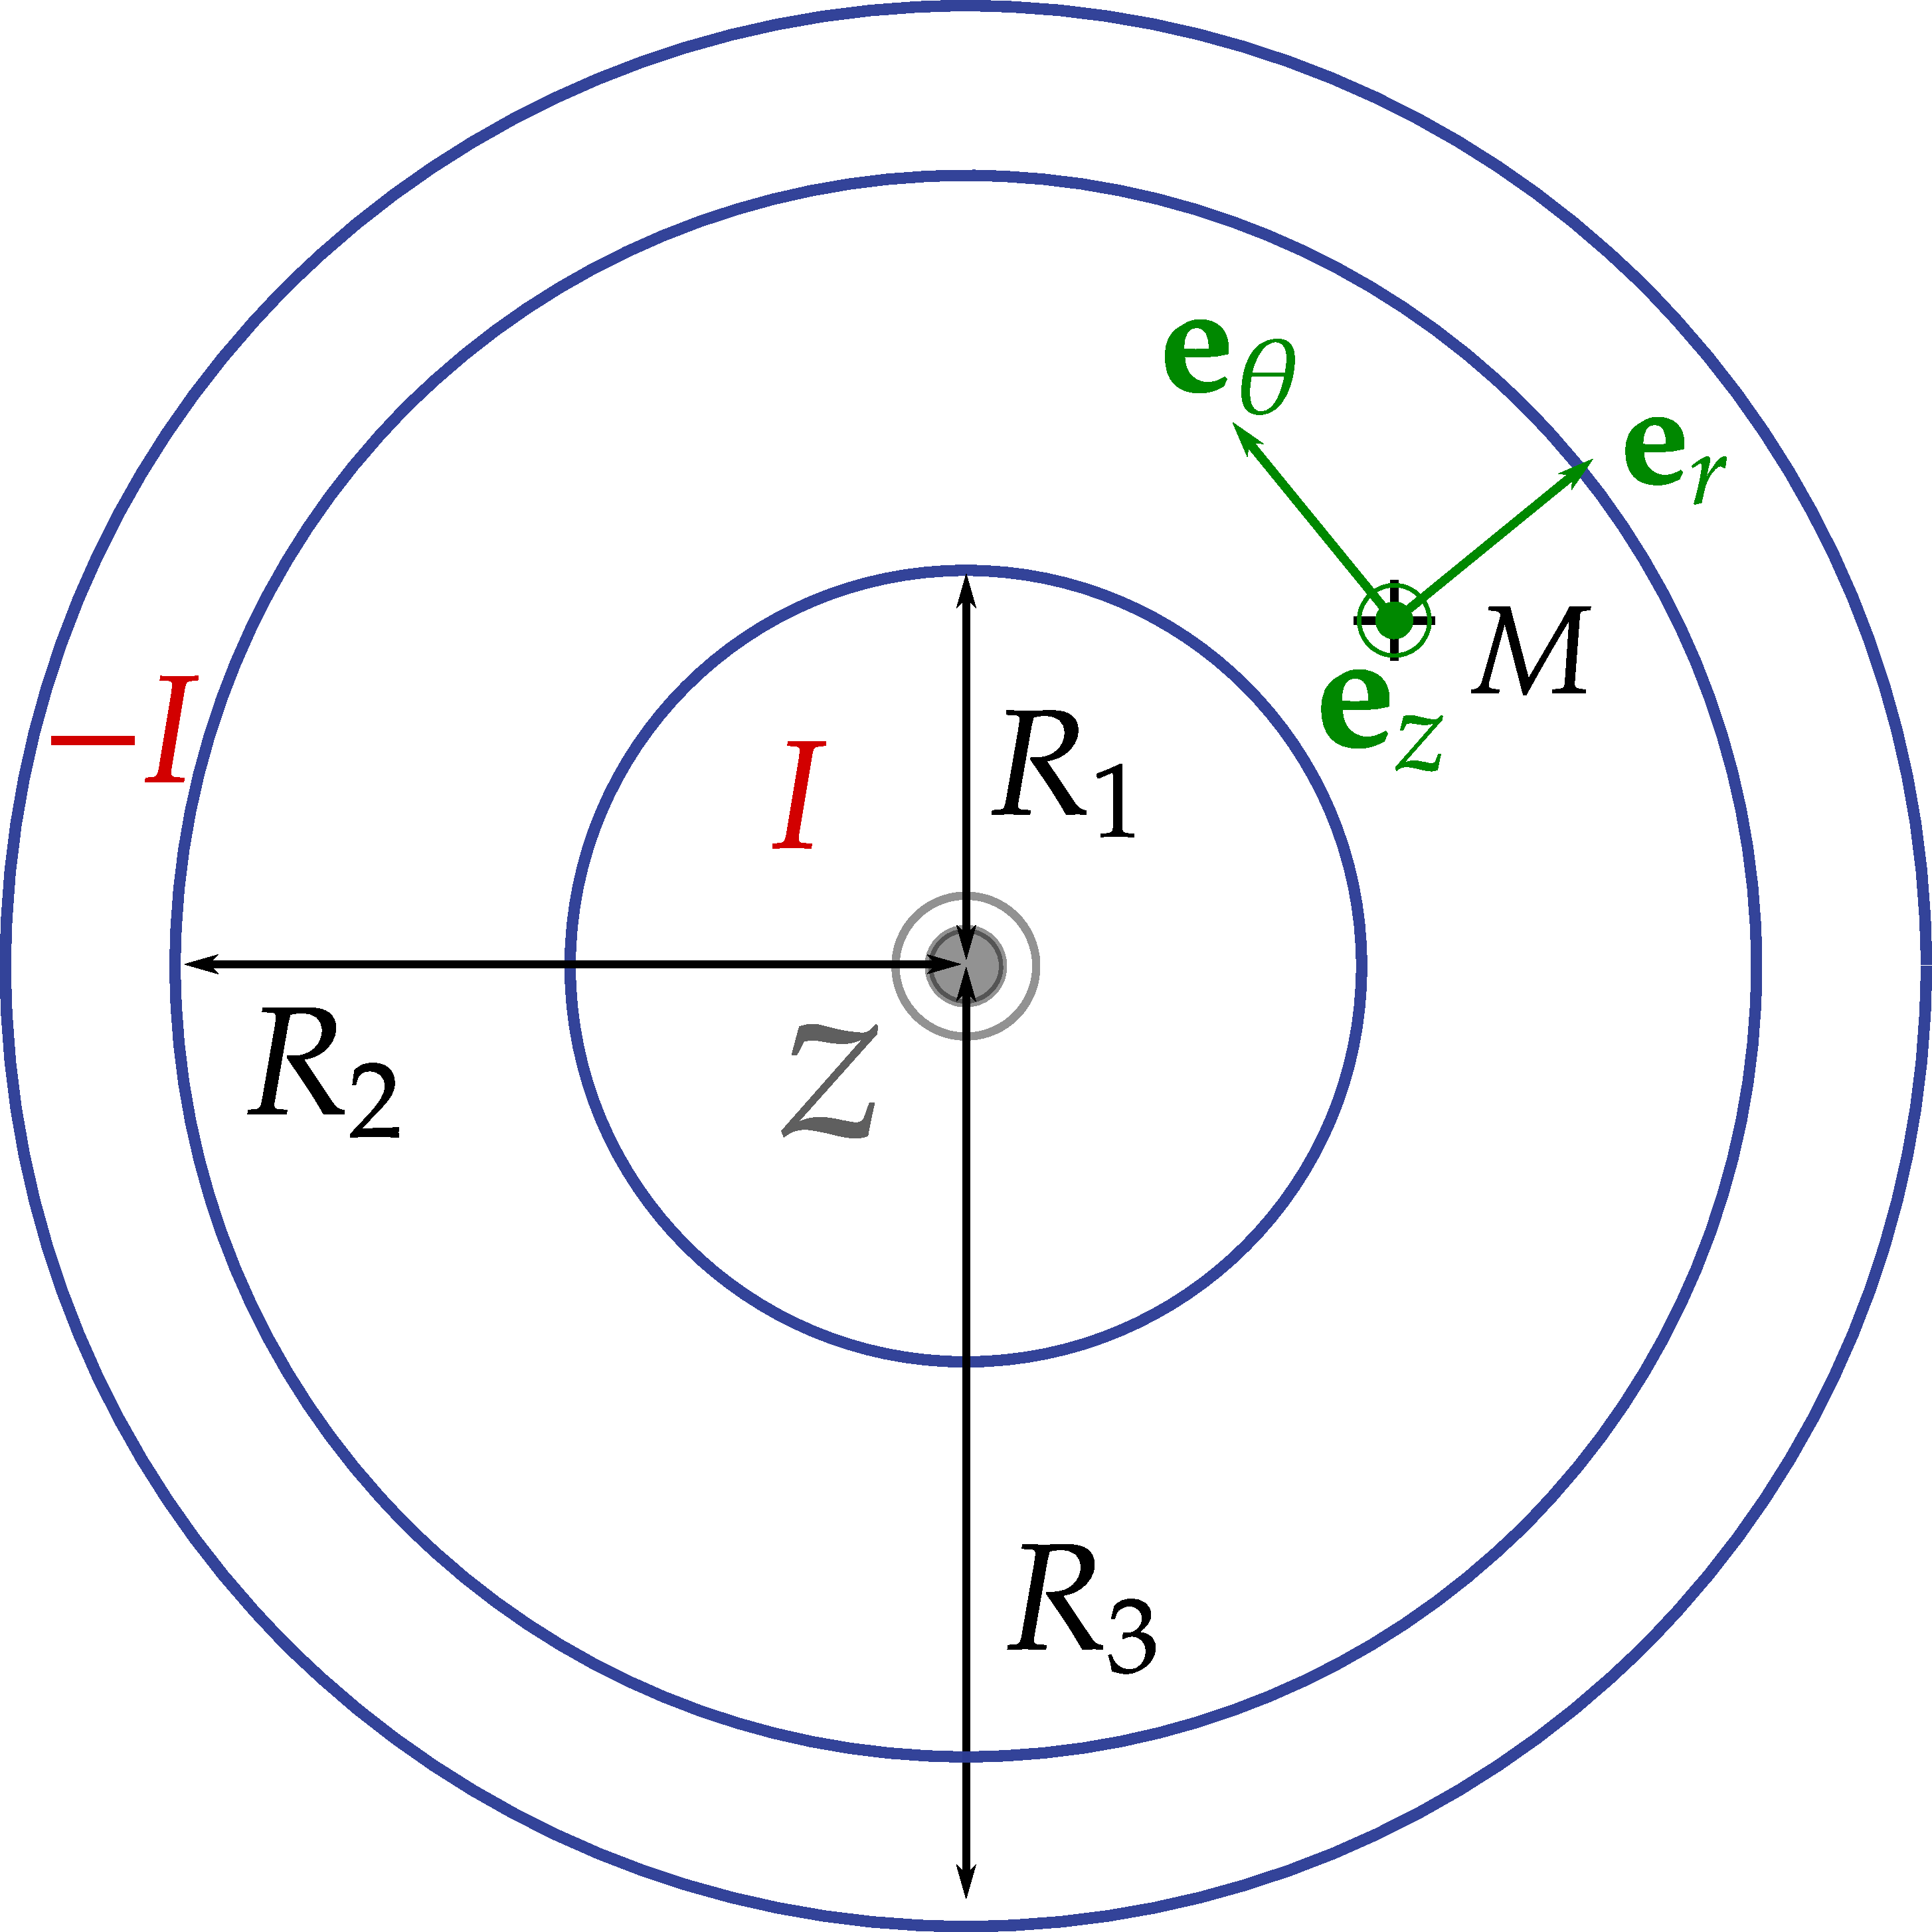
\includegraphics[scale=0.8]{coaxial}
		\caption{Coupe du câble coaxial dans le plan $(O, \er, \etheta)$.}
		\label{fig:magneto_coaxial}
	\end{figure}
	\item Sous sa forme la plus générale, le champ magnétique en $M$ 
	      s'écrit 
		      \begin{equation*}
			      \vecb(M) = B_r(M) \er + B_\theta(M) \etheta +
			      B_z(M) \ez.
		      \end{equation*}

		      \begin{description}
			     \item[Invariance:] La distribution de courant est 
			     invariante
			     \begin{itemize}
			     	\item par rotation autour de l'axe $(Oz)$, 
			     	      $\vecb$ ne dépend donc pas de $\theta$.
				\item par translation selon l'axe $(Oz)$, $\vecb$
				      ne dépend donc pas de $z$.
			     \end{itemize}
			      \item[Symétrie: ]
			      Le plan $(M, \er, \ez)$ est plan 
			      de symétrie de la distribution de 
			      courants. $\vecb(M)$ est donc 
			      orthogonal à ce plan et est donc colinéaire à
			      $\etheta$.
		      \end{description}
		     Finalement,
		     \begin{equation*}
			     \boxed{\vecb(M) = B(r) \etheta.}
		     \end{equation*}
	
	  \item Si $r > R_3$, le point $M$ se trouve à l'extérieur du câble 
		coaxial. Si on applique le théorème d'Ampère à un cercle 
		$\mathcal{C}$ de rayon $r$ et de centre $O$, cela donne
		\begin{equation*}
			\oint_\mathcal{C} \vecb \cdot \dl = \mu_0(I - I) = 0.
		\end{equation*}
		Ici, on $\dl = r \dtheta \etheta$ donc on obtient directement 
		\begin{equation*}
			\boxed{B(r) = 0}.
		\end{equation*}
		\fbox{Le champ magnétique est donc nul en dehors du câble.} Un câble 
		coaxial permet donc d'éviter de générer un champ magnétique parasite.

	\item   Les vecteurs densité de courant $\vecj_c$ et $\vecj_p$ sont réliés 
		à l'intensité $I$ du courant par les relations
		\begin{equation*}
			I = \iint_{S_c} \vecj_c \cdot \ds
			\quad \mathrm{et} \quad
			-I = \iint_{S_p} \vecj_p \cdot \ds,
		\end{equation*}
		où $S_c$ et $S_p$ sont respectivement les sections de la partie centrale
		et de la partie périphériques.
		Dans la partie centrale comme dans la partie périphérique, le
	        courant est uniforme. Les vecteurs densités de courant s'expriment
		donc
		\begin{equation*}
			\boxed{
			\vecj_c = \dfrac{I}{\pi R_1^2} \ez
			\quad \mathrm{et} \quad 
			\vecj_p = \dfrac{-I}{\pi \left(R_3^2 - R_2^2 \right)}
			\ez.
		}
		\end{equation*}

	\item On peut alors appliquer le théorème d'Ampère à un cercle $\mathcal{C}$
	      de rayon $r$ et de centre $O$
	      \begin{equation*}
		      \oint_\mathcal{C} \vecb \cdot \dl = I_\mathrm{enlacé},
	      \end{equation*}
	      où $I_\mathrm{enlacé}$ est le courant enlacé par $\mathcal{C}$.

	      On commence alors par exprimer le terme de gauche. On a $\dl = 
	      r \dtheta \etheta$ et donc le terme de gauche vaut $2 \pi r B(r)$.
	      Pour le terme de droite, c'est un peu plus compliqué. En effet, 3 cas
	      de figure se présentent

	      \begin{itemize}
		      \item Si $0 \le r \le R_1$, 
			    $I_\mathrm{enlacé} = \pi r^2 j_c = 
			    I\left(\dfrac{r}{R_1} \right)^2$.
		      \item Si $R_1 \le r \le R_2$, $I_\mathrm{enlacé} = I$.
		      \item Si $R_2 \le r \le R_3$, 
			    $I_\mathrm{enlacé} = 
			    I + \pi \left(R_3^2 - r^2\right) j_p =
			    I \left(1 - \dfrac{r^2 - R_2^2}{R_3^2 - R_2^2} \right)$.
	      \end{itemize}

	      Finalement, on obtient l'expression du champ magnétique en tout 
	      point $M$ de l'espace
	      \begin{equation*}
	      \boxed{
		     \vecb(M) = 
	      \left\{
		      \begin{array}{l}
			      \mathbf{0} \quad \mathrm{si} \quad r > R_3 \\[1em]
			      \dfrac{\mu_0 I}{2 \pi r} \left(1 - \dfrac{r^2 - R_2^2}
			      {R_3^2 - R_2^2} \right) \etheta \quad \mathrm{si} \quad
			      R_2 \le r \le R_3\\[1.5em]
			      \dfrac{\mu_0 I}{2 \pi r} \etheta \quad \mathrm{si} 
			      \quad R_1 \le r \le R_2\\[1em]
			      \dfrac{\mu_0 I}{2 \pi r}\left(\dfrac{r}{R_1}\right)^2
			      \etheta \quad \mathrm{si} \quad 0 \le r \le R_1.
		      \end{array}
		      \right.
	      }
	      \end{equation*}
\end{corrlist}
\end{corr}
